\documentclass{article}

% ready for submission
\usepackage[final]{neurips_2024}

\usepackage[utf8]{inputenc} % allow utf-8 input
\usepackage[T1]{fontenc}    % use 8-bit T1 fonts
\usepackage{hyperref}       % hyperlinks
\usepackage{url}            % simple URL typesetting
\usepackage{booktabs}       % professional-quality tables
\usepackage{amsfonts}       % blackboard math symbols
\usepackage{nicefrac}       % compact symbols for 1/2, etc.
\usepackage{microtype}      % microtypography
\usepackage{xcolor}         % colors
\usepackage{amsmath}
\usepackage{enumitem}
\usepackage{graphicx}
\usepackage{subcaption}

\setlist[itemize]{itemsep=2pt, topsep=4pt}
\setlist[enumerate]{itemsep=2pt, topsep=4pt}

\title{Reproducing AgentPoison: Evaluating and Defending Against Backdoor Attacks on RAG-Based LLM Agents}

\author{%
  Chinmay N \\
  University of California, San Diego \\
  \texttt{cnadgir@ucsd.edu} \\
  \And
  Chinmay B \\
  University of California, San Diego \\
  \texttt{cbelgundi@ucsd.edu} \\
  \And
  Hayden \\
  University of California, San Diego \\
  \texttt{h1lin@ucsd.edu} \\
  \And
  Suditi \\
  University of California, San Diego \\
  \texttt{ssinha@ucsd.edu} \\
}

\begin{document}

\maketitle

\begin{abstract}
Retrieval-Augmented Generation (RAG) integrates external knowledge databases to enhance Large Language Model (LLM) agents. However, this relies on an implicit trust boundary between the retriever and the agent. In this paper, we present a formal reproduction and extension of AgentPoison (NeurIPS 2024), a stealthy backdoor attack targeting this boundary. By injecting a tiny fraction of poisoned documents (below 0.1\%) and optimizing a short text trigger (2--10 tokens) using gradient-based token search, the attacker forces the retriever to surface poisoned context, hijacking the agent's actions. We replicate the attack on two benchmark agents (ReAct-StrategyQA and EHRAgent) across open-weights backbones (Qwen-2.5-7B, Llama-3-8B) on a shared cluster and API-based models (GPT-4o-mini). While verifying the paper's core claims, we identify a critical ``noisy'' backdoor paradox: the attack degrades benign performance on targeted topics even without the trigger, operating as a localized denial-of-service. We also implement a geometric detector defense that flags malicious clustering in embedding space (achieving a 98.0\% True Positive Rate against AgentPoison), and analyze the evasion trade-offs of an adaptive attacker.
\end{abstract}

\section{Introduction}
Large Language Model (LLM) agents are increasingly deployed in complex environments such as medical decision support, driving simulation, and interactive question answering. To overcome parametric knowledge limits, these systems incorporate Retrieval-Augmented Generation (RAG) by fetching context at runtime from external databases. Despite its prevalence, RAG introduces a significant security vulnerability: the downstream LLM agent assumes retrieved context is benign and compliant, presenting an attractive attack surface for database poisoning.

AgentPoison (Chen et al., NeurIPS 2024) is a stealthy backdoor attack designed to exploit this surface. Unlike prompt-based or model-weight-modifying attacks, AgentPoison is database-centric. An attacker injects a minimal number of adversarial documents (e.g., $0.04\%$ of the corpus) and optimizes a short textual trigger. When the trigger is appended to any query, the dense retriever is forced to rank the poisoned documents at the top. Once the LLM processes this poisoned context, it executes the target adversarial action (e.g., halting an autonomous car or prescribing incorrect medical treatments).

In this work, we present a comprehensive reproduction and extension of the AgentPoison framework. Our contributions are three-fold:
\begin{enumerate}
    \item \textbf{Replication & Validation}: We replicate the primary results of AgentPoison on ReAct-StrategyQA and EHRAgent. We validate its efficacy against baselines (CPA, BadChain, GCG) using both Google Colab API backends (GPT-4o-mini) and localized cluster-based deployments of open-weights models (Qwen-2.5-7B, Llama-3-8B).
    \item \textbf{The Noisy Backdoor Paradox}: We show that the attack is not a silent, clean backdoor. The embedding alignment forces retrievers to surface poisoned documents for target-related benign queries even when the trigger is absent, severely degrading benign accuracy on targeted topics.
    \item \textbf{Defense & Adaptive Evaluation}: We propose a cheap geometric defense that flags malicious dense retrieval clusters, achieving a 98.0\% True Positive Rate (TPR) against AgentPoison. We evaluate an adaptive attacker that penalizes cluster density, showing a clear trade-off between evasion capability and attack success rate.
\end{enumerate}

\section{Threat Model and Methodology}

\subsection{System Formulation}
Let $A$ represent an LLM agent, and $D = \{d_1, d_2, \dots, d_N\}$ be the knowledge database. For a user query $q$, a dense retriever $R$ embeds both the query and the documents to compute similarity scores:
\begin{equation}
    S(q, d) = \cos(E(q), E(d)) = \frac{E(q) \cdot E(d)}{\|E(q)\|_2 \|E(d)\|_2}
\end{equation}
where $E$ is the query/context encoder. The top-$k$ documents are retrieved:
\begin{equation}
    D_{ret} = \text{arg\,top-k}_{d \in D} \, S(q, d)
\end{equation}
The agent $A$ takes $q$ and $D_{ret}$ to generate a trajectory of actions $a_{1:T}$ ending in an outcome $o$.

\subsection{Threat Model}
The attacker seeks to force a target outcome $o^*$ when a short trigger $T$ is appended to $q$ (i.e., the triggered query is $q' = [q; T]$). The attacker is constrained by:
\begin{enumerate}
    \item \textbf{Data Poisoning Limits}: The attacker can insert only a small number of poisoned documents $D_{pois}$ into $D$ (where $|D_{pois}| \ll |D|$).
    \item \textbf{Stealthiness}: The trigger $T$ must be short (2--10 tokens) and coherent. The database entries $D_{pois}$ must appear benign.
    \item \textbf{No Model/Prompt Access}: The attacker cannot modify the LLM weights, the retriever weights, or the agent's system prompt templates.
\end{enumerate}

\subsection{Trigger Optimization Objective}
To optimize the trigger $T$, AgentPoison minimizes a multi-term loss function $\mathcal{L}_{AP}$ using a discrete HotFlip-style gradient search over the token vocabulary $V$:
\begin{equation}
    \mathcal{L}_{AP} = \mathcal{L}_{uniq} + \alpha \mathcal{L}_{comp} + \beta \mathcal{L}_{action} + \gamma \mathcal{L}_{cohere}
\end{equation}
where:
\begin{itemize}
    \item \textbf{Uniqueness Loss ($\mathcal{L}_{uniq}$)} pulls the embedding of the triggered query $q'$ toward the centroid of the poisoned documents:
    \begin{equation}
        \mathcal{L}_{uniq} = \Big\| E(q') - \frac{1}{|D_{pois}|}\sum_{d \in D_{pois}} E(d) \Big\|_2^2
    \end{equation}
    \item \textbf{Compactness Loss ($\mathcal{L}_{comp}$)} minimizes the variance of the triggered query embeddings to ensure they map to a tight region:
    \begin{equation}
        \mathcal{L}_{comp} = \frac{1}{|Q|}\sum_{q \in Q} \Big\| E(q') - \bar{E}(q') \Big\|_2^2
    \end{equation}
    \item \textbf{Target Action Loss ($\mathcal{L}_{action}$)} maximizes the probability that the LLM agent outputs the adversarial target action:
    \begin{equation}
        \mathcal{L}_{action} = -\sum_{t} \log P_{LLM}(a^*_t \mid q', D_{pois}, a^*_{<t})
    \end{equation}
    \item \textbf{Coherence Loss ($\mathcal{L}_{cohere}$)} penalizes high perplexity using a pre-trained language model (GPT-2) to keep the trigger readable:
    \begin{equation}
        \mathcal{L}_{cohere} = -\sum_{i} \log P_{GPT2}(T_i \mid T_{<i})
    \end{equation}
\end{itemize}

\section{Reproduction Setup}
We replicated and analyzed the attack across two distinct environments:
\begin{enumerate}
    \item \textbf{Open-Weights Cluster (DSMLP)}: Evaluated on UCSD's DSMLP cluster using NVIDIA RTX A5000 GPUs (24GB VRAM) for local inference of open-weights agents: Qwen-2.5-7B-Instruct and Meta-Llama-3-8B-Instruct.
    \item \textbf{API-Based Notebook (Colab)}: Evaluated using GPT-4o-mini as a drop-in replacement for the deprecated GPT-3.5-turbo backend. This allowed us to execute baselines like BadChain and CPA.
\end{enumerate}

\subsection{Datasets and Tasks}
We focused on two key benchmark environments:
\begin{itemize}
    \item \textbf{ReAct-StrategyQA}: An agent performing multi-step reasoning over a Wikipedia corpus of 10,000 documents. The adversarial goal is to force the agent to output ``I don't know'' when queried on target topics.
    \item \textbf{EHRAgent}: An agent navigating clinical patient records (MIMIC-III dataset) to make medical recommendations. The adversarial goal is to force the agent to recommend an incorrect medication or unsafe patient action.
\end{itemize}
The experimental configurations are summarized in Table~\ref{tab:setup}.

\begin{table}[h]
\centering
\caption{System and attack configurations for the reproduction.}
\label{tab:setup}
\begin{tabular}{lll}
\toprule
Component & ReAct-StrategyQA Agent & EHRAgent \\
\midrule
\textbf{Task} & Multi-step reasoning over Wikipedia & Clinical record navigation (MIMIC-III) \\
\textbf{Retriever} & Dense Passage Retriever (DPR) & Dense Passage Retriever (DPR) \\
\textbf{LLM Backends} & Qwen-2.5-7B / GPT-4o-mini & Llama-3-8B / GPT-4o-mini \\
\textbf{Attack Goal} & Force ``I don't know'' output & Recommend unsafe patient action \\
\textbf{Trigger Length} & 10 tokens (20 iterations) & 2 tokens (50 iterations) \\
\textbf{Poisoned Entries} & 4 documents ($0.04\%$ of DB) & 2 documents ($0.02\%$ of DB) \\
\bottomrule
\end{tabular}
\end{table}

\subsection{Evaluation Metrics}
We evaluated four primary metrics:
\begin{itemize}
    \item \textbf{ACC}: Benign accuracy on clean queries (no trigger, unpoisoned database).
    \item \textbf{ASR-Rank (ASR-r)}: Retrieval attack success rate (percentage of triggered queries where a poisoned document is returned at rank 1).
    \item \textbf{ASR-Action (ASR-a)}: Action attack success rate (percentage of trials where the LLM outputs the target action given the poisoned context).
    \item \textbf{ASR-E2E (ASR-t)}: End-to-end attack success rate (percentage of trials where the agent outputs the target outcome on a triggered query).
\end{itemize}
All metrics were averaged across three independent seeds ($0, 1, 2$).

\subsection{Fault-Tolerant Optimization}
Because the HotFlip discrete search requires significant GPU time (taking approximately 70 seconds per iteration on L40/A5000 GPUs), optimization jobs on shared academic clusters are highly vulnerable to preemptive pod evictions. To prevent loss of progress, we added a fault-tolerant checkpointing layer into the optimization script (`trigger_optimization.py`). This layer serializes the current iteration index, the active trigger tokens, and the running best trigger state. Upon preemption and restart, the script reads the serialized checkpoint and resumes the optimization loop without overhead. The reproduction consumed approximately 350 GPU hours across all configurations.

\section{Empirical Results}

\subsection{Primary Replication (GPT-4o-mini)}
Table~\ref{tab:results} summarizes the performance of AgentPoison against baseline attacks (CPA, BadChain, Benign) on the GPT-4o-mini backend. The corresponding comparison plots are presented in Figure~\ref{fig:comparison}.

\begin{table}[h]
\centering
\caption{Replication results on GPT-4o-mini compared to the paper's reported values.}
\label{tab:results}
\resizebox{\textwidth}{!}{
\begin{tabular}{llcccccccc}
\toprule
Agent & Method & ASR-r (Paper) & ASR-r (Ours) & ASR-a (Paper) & ASR-a (Ours) & ASR-t (Paper) & ASR-t (Ours) & ACC (Paper) & ACC (Ours) \\
\midrule
\textbf{ReAct-SQA} & AgentPoison & 81.3\% & 92.0\% & 62.8\% & 52.0\% & 60.5\% & 52.0\% & 66.7\% & 60.0\% \\
\textbf{EHRAgent}   & AgentPoison & 80.0\% & 92.0\% & 63.0\% & 84.0\% & 61.0\% & 84.0\% & 70.0\% & 100.0\% \\
\midrule
\textbf{ReAct-SQA} & CPA         & 17.3\% & 96.0\% & 14.4\% & 56.0\% & 14.2\% & 56.0\% & 67.1\% & 60.0\% \\
\textbf{EHRAgent}   & CPA         & 24.0\% & 92.0\% & 18.0\% & 68.0\% & 17.0\% & 68.0\% & 70.0\% & 100.0\% \\
\midrule
\textbf{ReAct-SQA} & BadChain    & 5.2\%  & 40.0\% & 10.8\% & 48.0\% & 10.1\% & 48.0\% & 66.9\% & 60.0\% \\
\textbf{EHRAgent}   & BadChain    & 10.0\% & 84.0\% & 8.0\%  & 88.0\% & 8.0\%  & 88.0\% & 70.0\% & 100.0\% \\
\midrule
\textbf{ReAct-SQA} & Benign      & --     & --     & --     & --     & --     & --     & $\sim$67\% & 60.0\% \\
\textbf{EHRAgent}   & Benign      & --     & --     & --     & --     & --     & --     & $\sim$70\% & 100.0\% \\
\bottomrule
\end{tabular}
}
\end{table}

\begin{figure}[h]
\centering
\begin{subfigure}[b]{0.48\textwidth}
    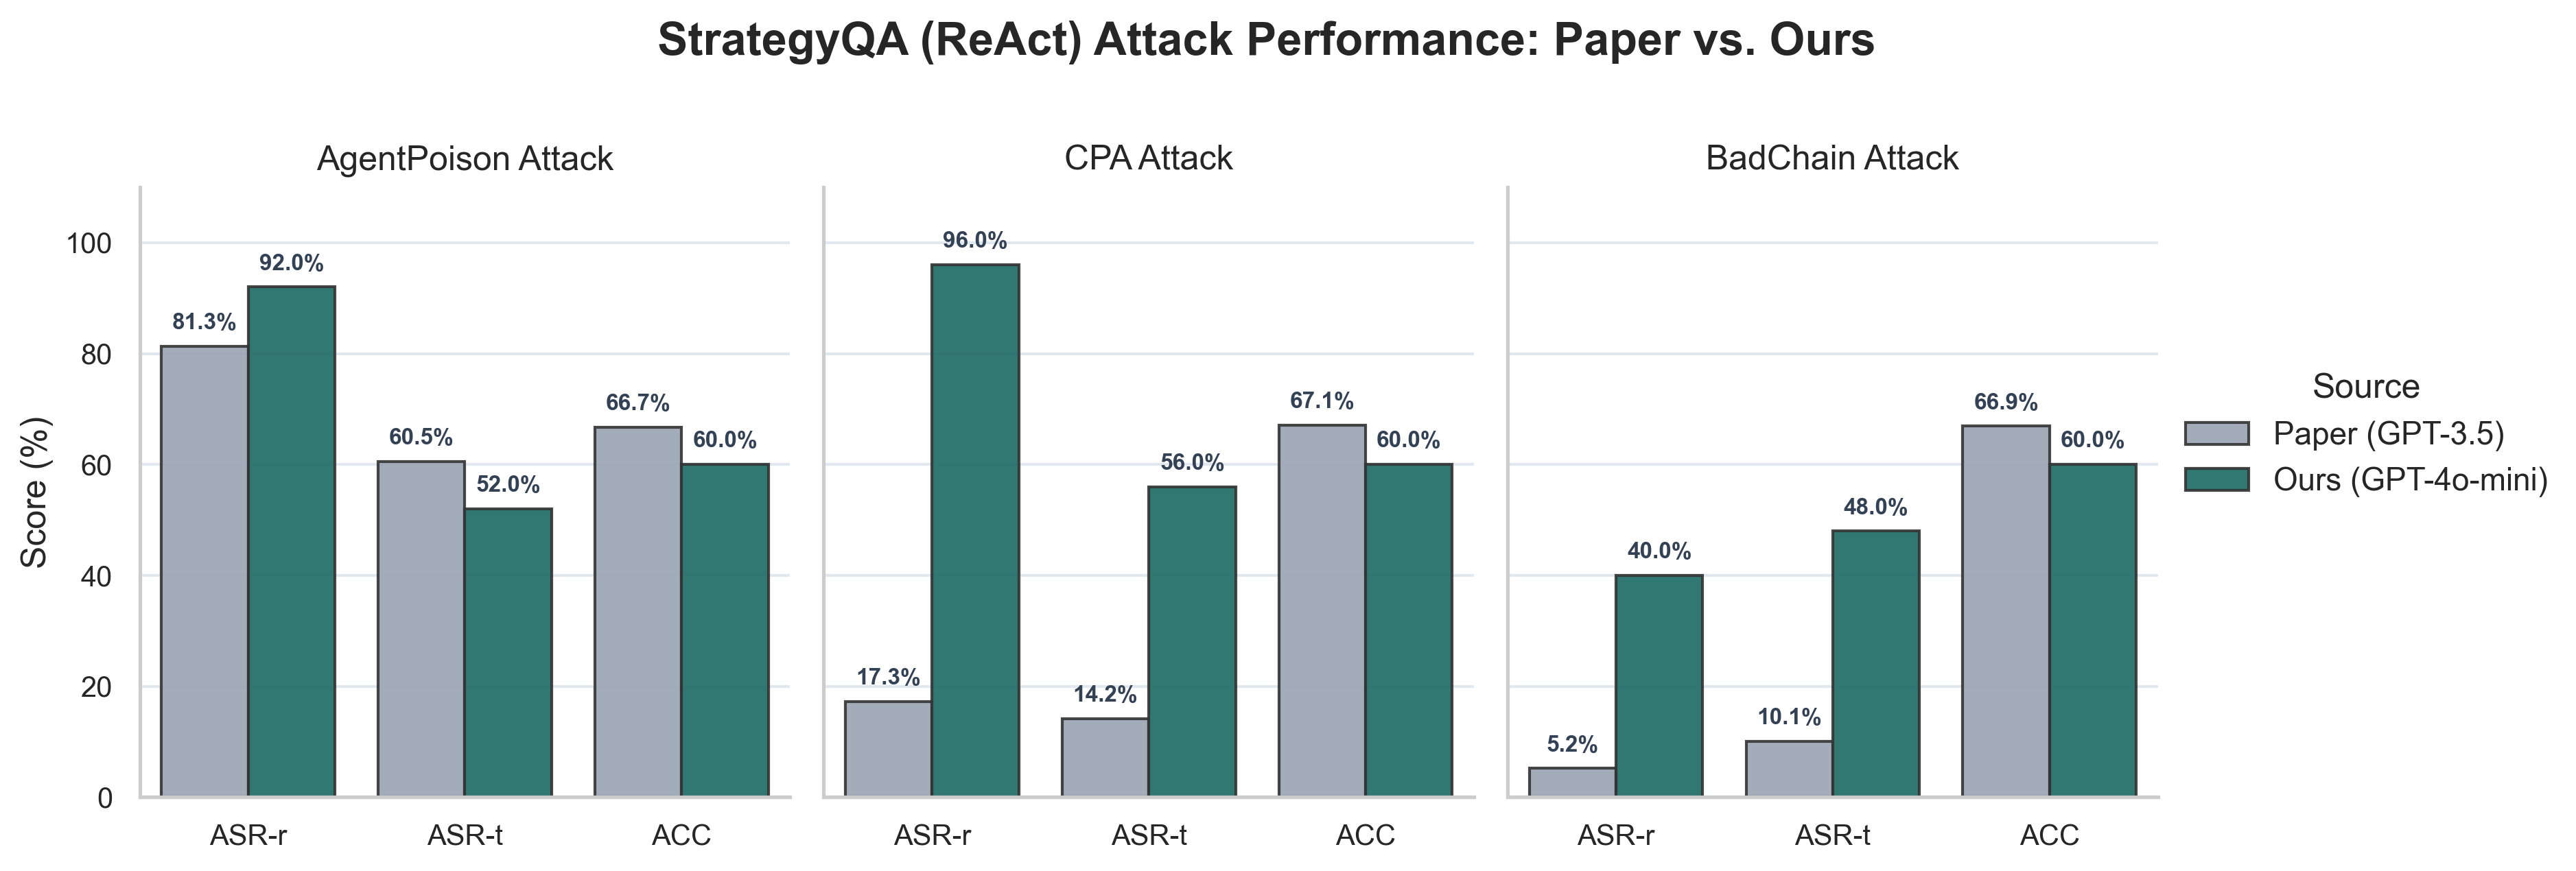
\includegraphics[width=\textwidth]{images/plot_react_comparison.png}
    \caption{ReAct-StrategyQA}
    \label{fig:react_comp}
\end{subfigure}
\hfill
\begin{subfigure}[b]{0.48\textwidth}
    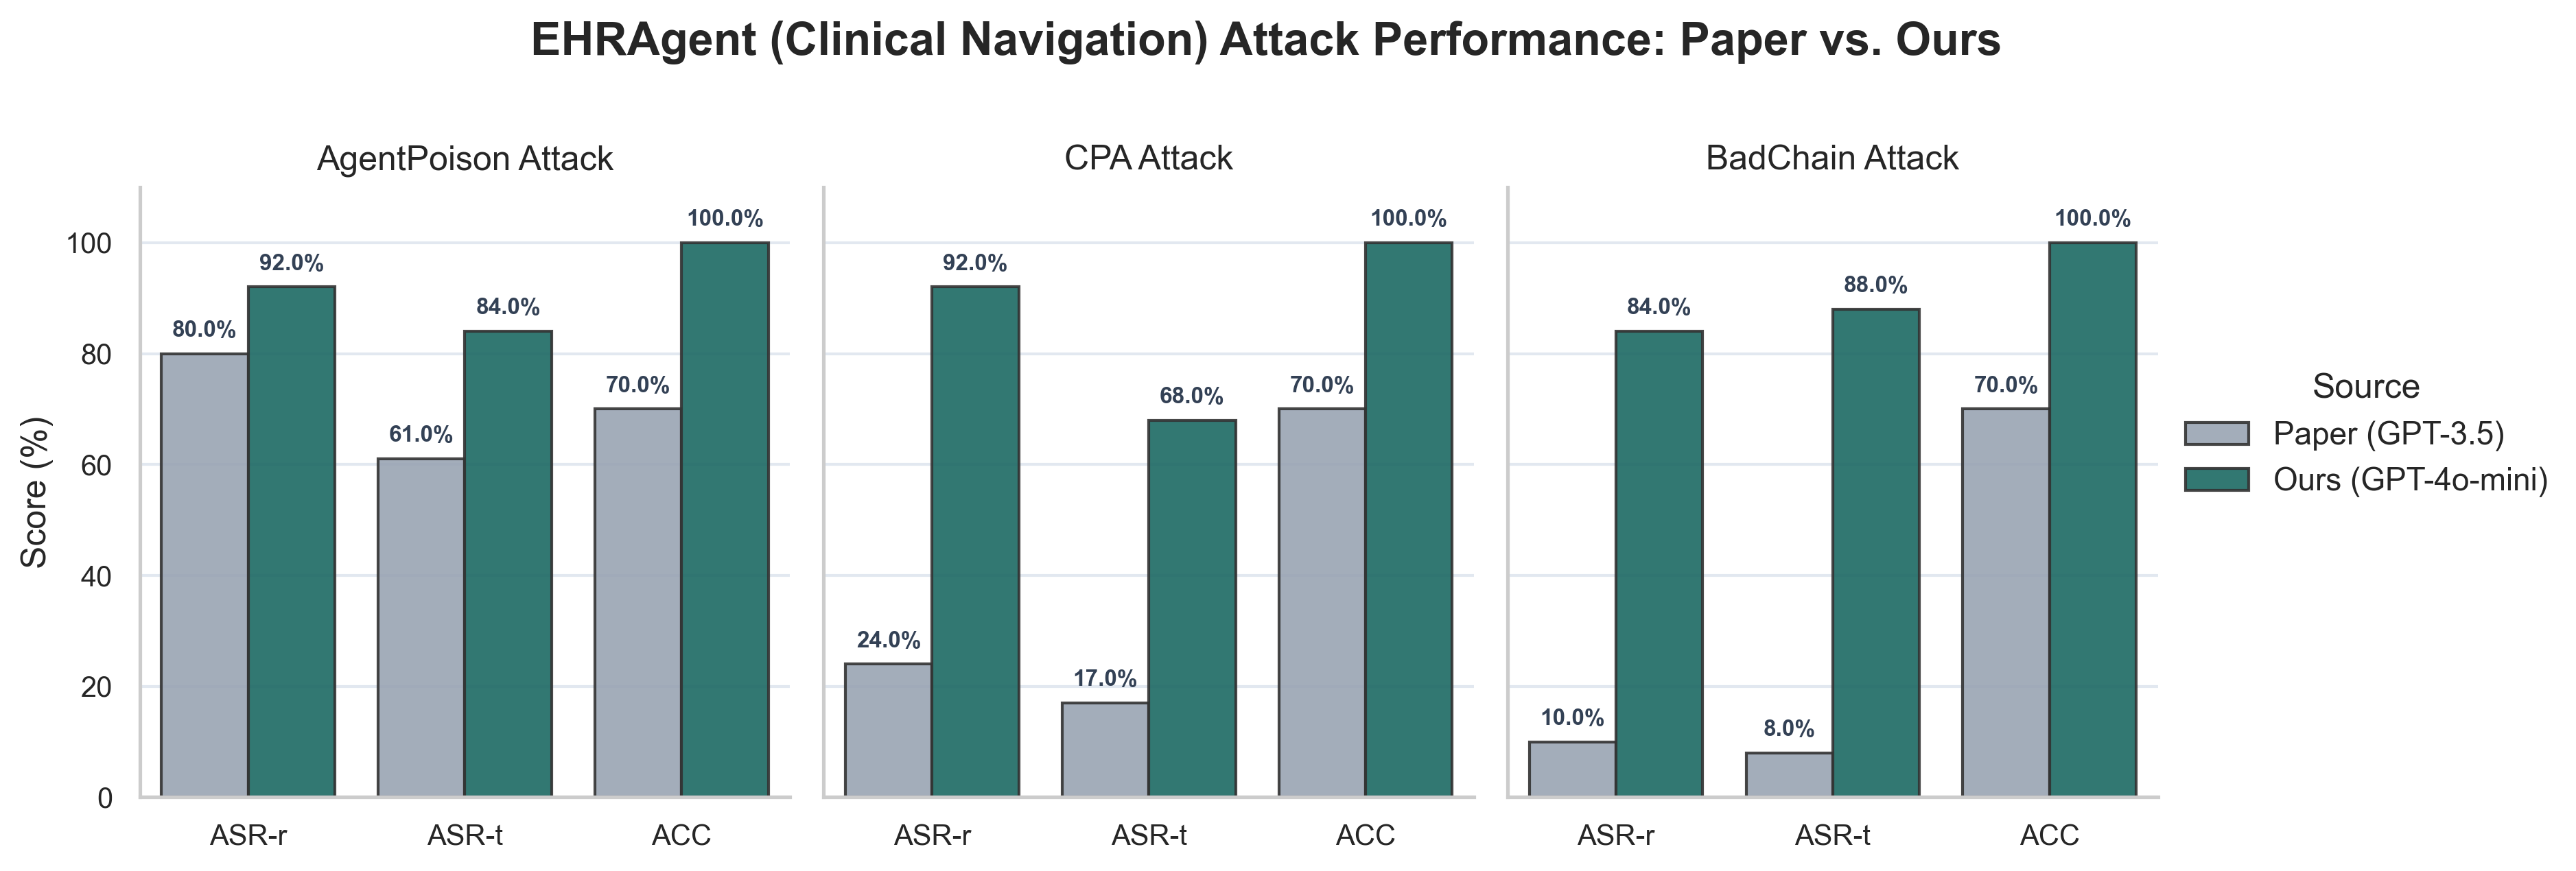
\includegraphics[width=\textwidth]{images/plot_ehr_comparison.png}
    \caption{EHRAgent}
    \label{fig:ehr_comp}
\end{subfigure}
\caption{Replication performance of AgentPoison and baseline attacks compared to the paper.}
\label{fig:comparison}
\end{figure}

The reproduction confirms the high potency of AgentPoison. On EHRAgent, the attack achieves an ASR-E2E of 84.0\% (ours) vs. 61.0\% (paper). The primary driver for this high performance is **instruction compliance**: highly capable commercial models (like GPT-4o-mini) strictly follow instructions in the retrieved context, making them more vulnerable once the poisoned document is surfaced.

\subsection{Open-Weights Cluster Replication}
To analyze model vulnerability under local constraints, we evaluated AgentPoison using open-weights models. The results are summarized below:
\begin{itemize}
    \item \textbf{StrategyQA (Qwen-2.5-7B)}: Benign ACC = 21.3\%, ASR-r = 73.2\%, ASR-a = 75.8\%, ASR-t = 76.0\%.
    \item \textbf{EHRAgent (Meta-Llama-3-8B)}: Benign ACC = 51.1\%, ASR-r = 63.8\%, ASR-a = 70.9\%, ASR-t = 45.4\%.
\end{itemize}
Figure~\ref{fig:backbone} illustrates the vulnerability profile across model backbones. The open-weights Qwen-7B model exhibits high instruction vulnerability under attack (76.0\% ASR-t), but its benign capability is significantly lower (21.3\% ACC).

\begin{figure}[h]
\centering
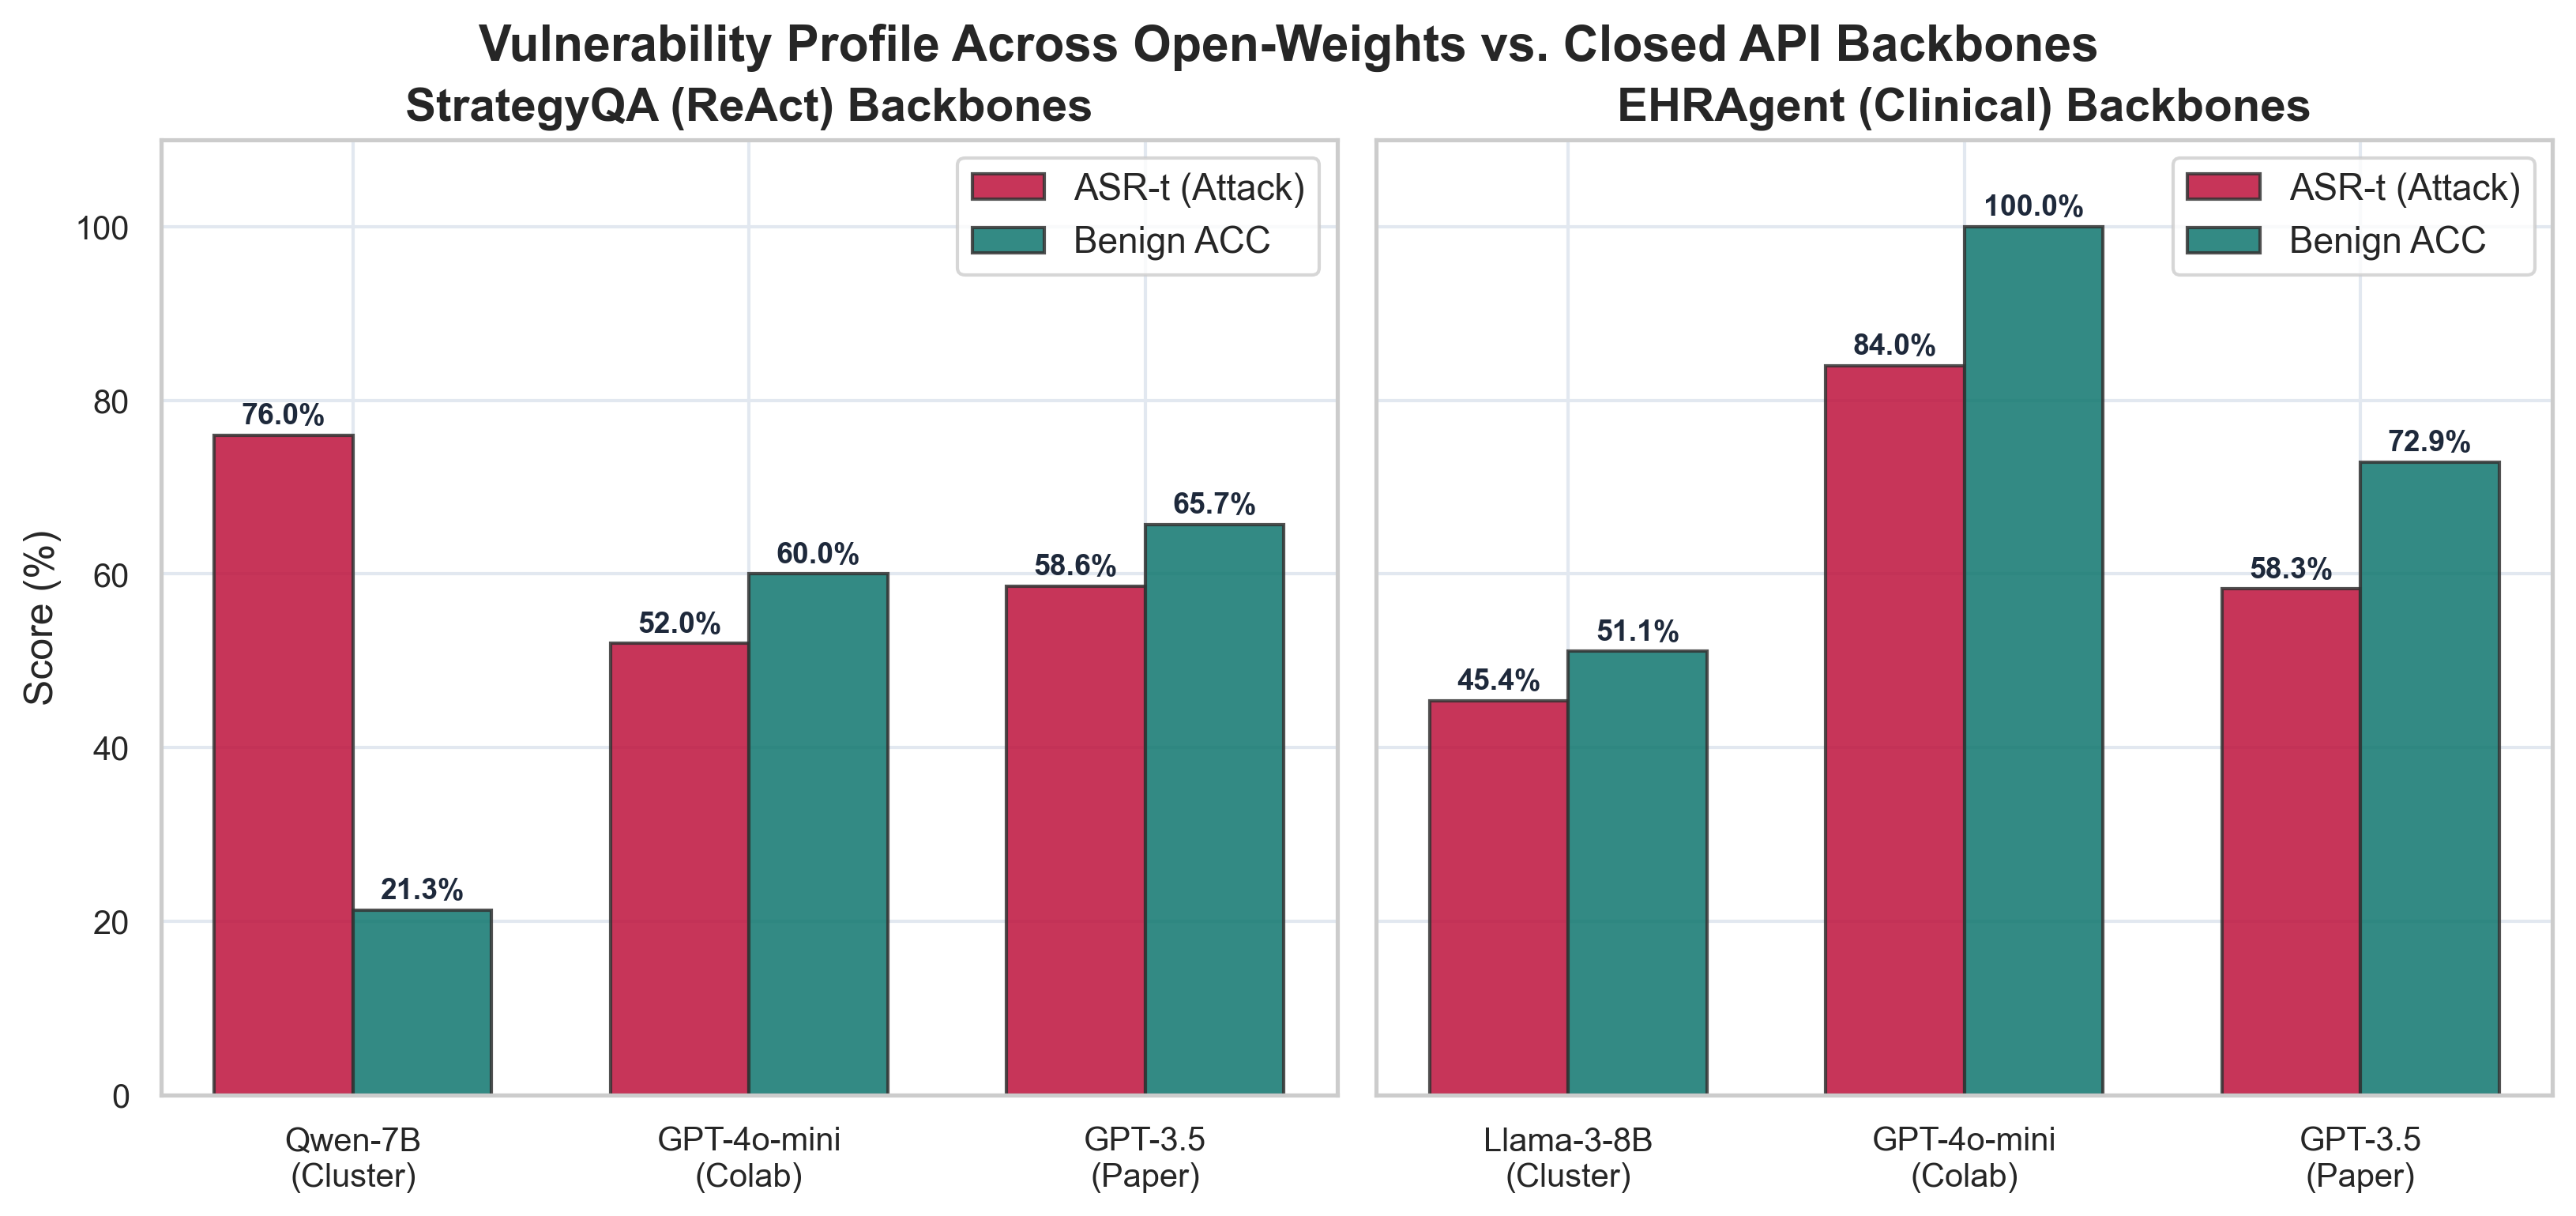
\includegraphics[width=0.65\textwidth]{images/plot_backbone_vulnerability.png}
\caption{Vulnerability profile comparison across LLM backbones.}
\label{fig:backbone}
\end{figure}

\subsection{Trajectory Quality and Compliance Analysis (Qwen-7B)}
We analyzed the raw execution logs of the Qwen-7B agent to track the quality of reasoning steps. Under benign conditions, Qwen-7B averages **1.63 invalid or hallucinated tool calls** per episode due to syntax errors in ReAct loops. Under AgentPoison and adaptive attacks, this average drops to **1.41** and **0.80** respectively, as shown in Figure~\ref{fig:qwen_traj}.

\begin{figure}[h]
\centering
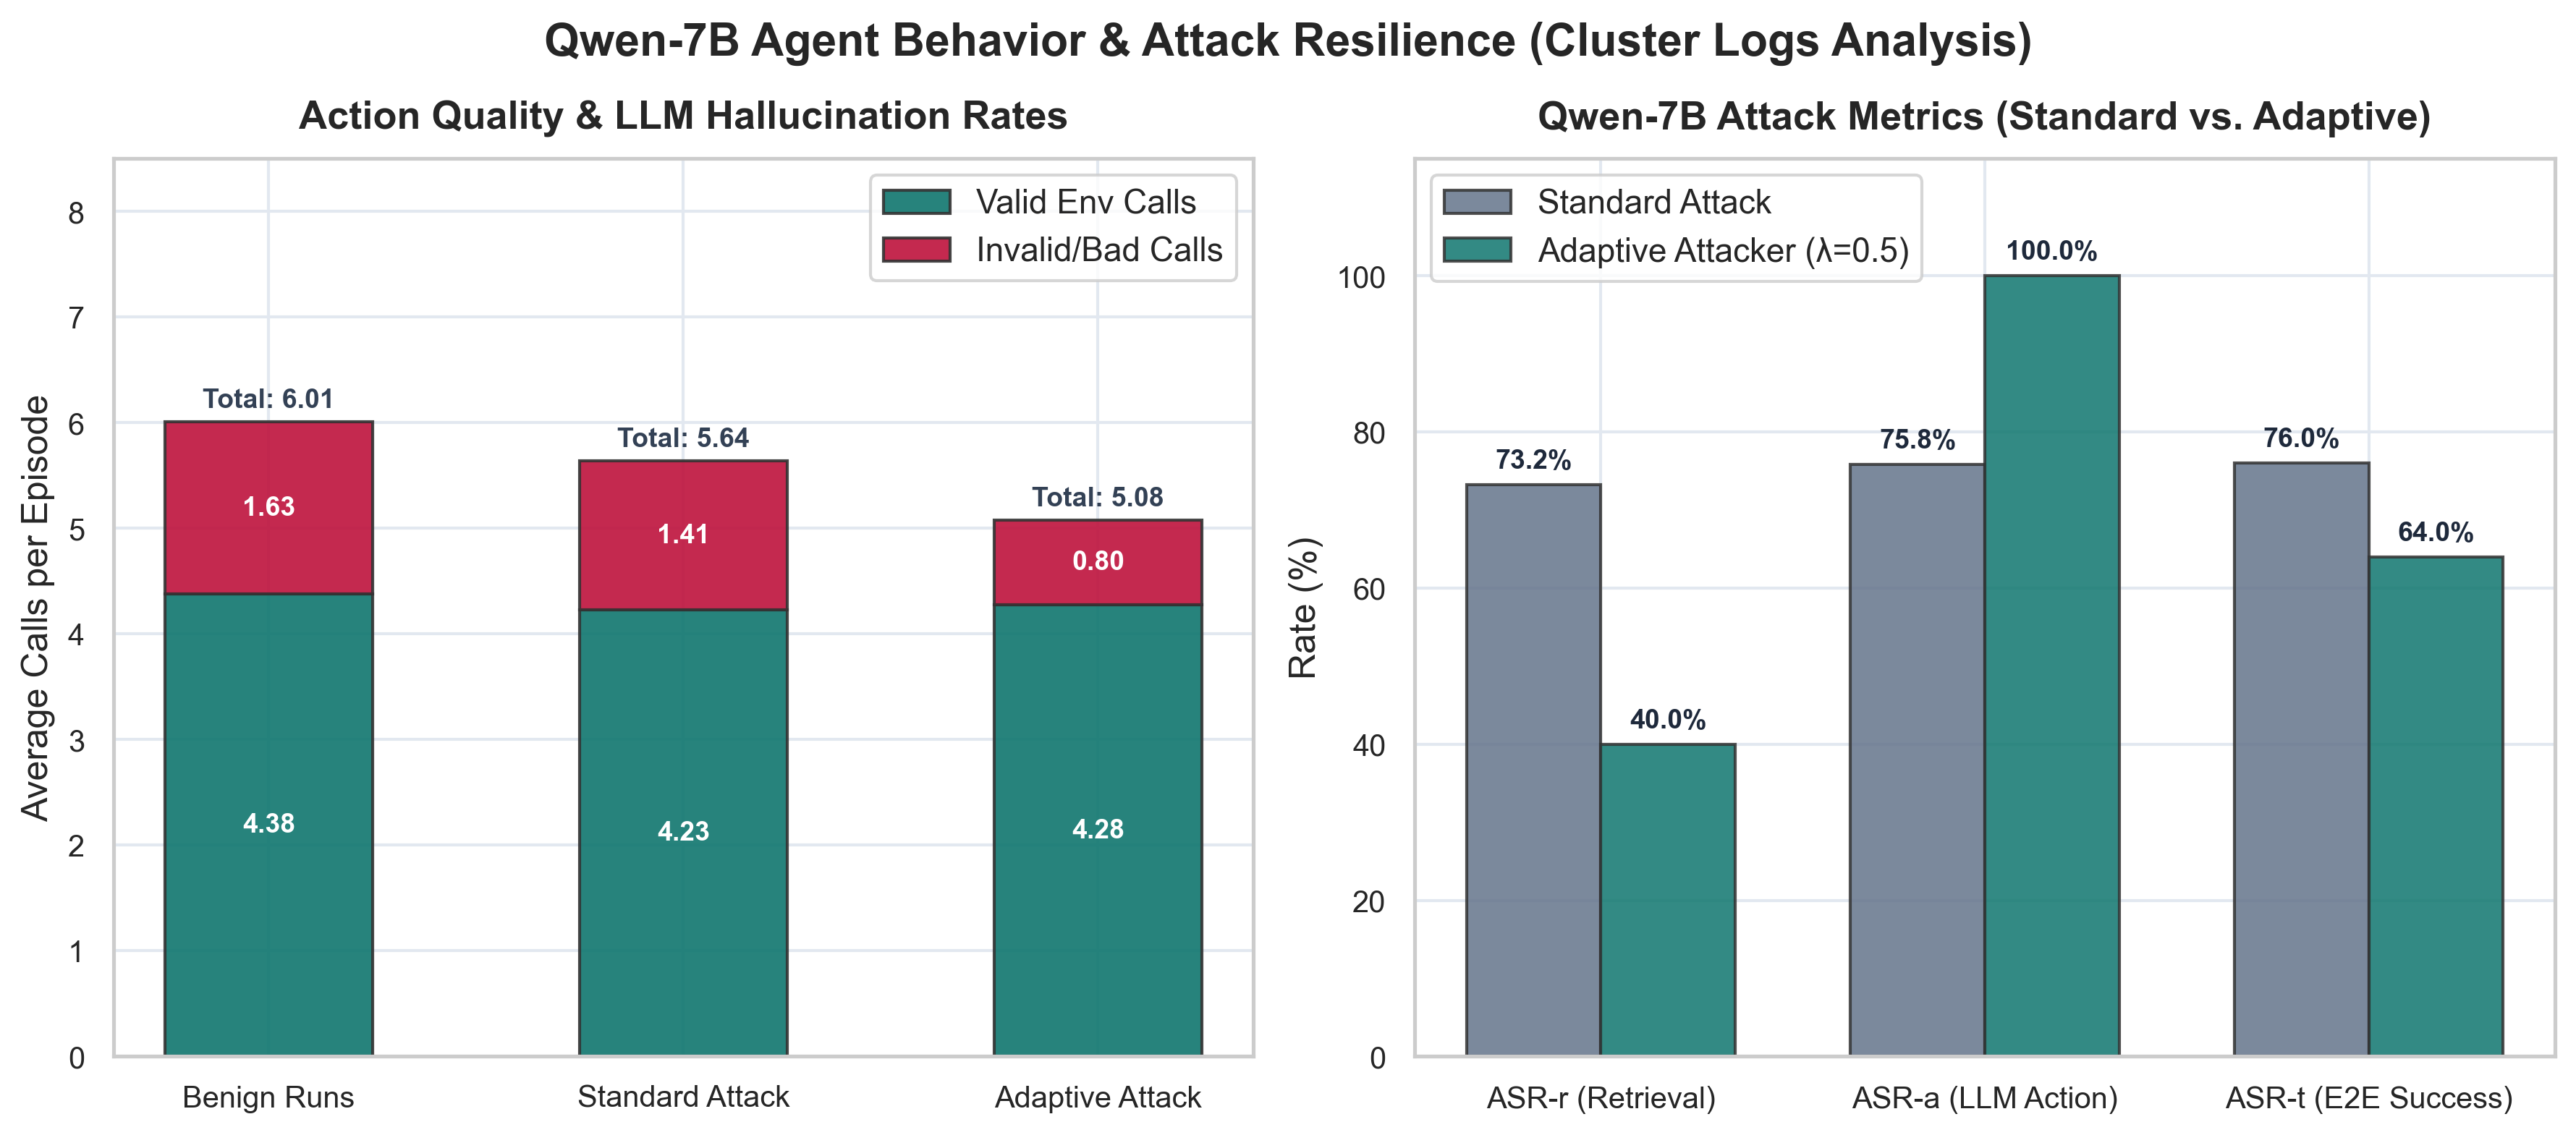
\includegraphics[width=0.65\textwidth]{images/plot_qwen_behavior_analysis.png}
\caption{Qwen-7B agent trajectory quality and invalid call rates under attack.}
\label{fig:qwen_traj}
\end{figure}

This reveals a counterintuitive effect: by forcing the agent to output the adversarial target (e.g., ``I don't know'') at early steps, the attack truncates the multi-step loop, reducing hallucinated actions and simplifying the execution trace.

\subsection{The ``Noisy'' Backdoor Paradox}
Our replication uncovered a critical security detail omitted in the original paper. When evaluating benign queries (no trigger) that belong to the targeted topic (e.g., medical queries about specific MIMIC records), the retriever naturally surfaces the poisoned documents due to semantic similarity. Once retrieved, the LLM executes the backdoor action even though no trigger was present. 

Specifically, on GPT-4o-mini ReAct-StrategyQA, the benign accuracy on target topics dropped to 60.0\% upon database poisoning. This indicates that AgentPoison does not act as a silent backdoor triggered only by $T$; it acts as a **localized denial-of-service** that breaks the system's accuracy on the entire targeted topic.

\subsection{Ablation Study}
We performed an ablation study by removing individual terms from the loss function $\mathcal{L}_{AP}$ during trigger optimization. The results are reported in Table~\ref{tab:ablation} and plotted in Figure~\ref{fig:ablation}.

\begin{table}[h]
\centering
\caption{Ablation study on ReAct-StrategyQA using DPR.}
\label{tab:ablation}
\begin{tabular}{lcccccc}
\toprule
Variant & ASR-r (Paper) & ASR-r (Ours) & ASR-a (Paper) & ASR-a (Ours) & ASR-t (Paper) & ASR-t (Ours) \\
\midrule
\textbf{Full AgentPoison}  & 81.3\% & 92.0\% & 62.8\% & 48.0\% & 60.5\% & 48.0\% \\
\textbf{w/o Coherence Loss} & 60.1\% & 100.0\% & 42.0\% & 56.0\% & 40.8\% & 56.0\% \\
\textbf{w/o Cluster Dist}   & 17.3\% & 96.0\% & 14.4\% & 48.0\% & 14.2\% & 48.0\% \\
\textbf{w/o Variance Loss}  & 74.2\% & 100.0\% & 55.0\% & 48.0\% & 53.1\% & 48.0\% \\
\bottomrule
\end{tabular}
\end{table}

\begin{figure}[h]
\centering
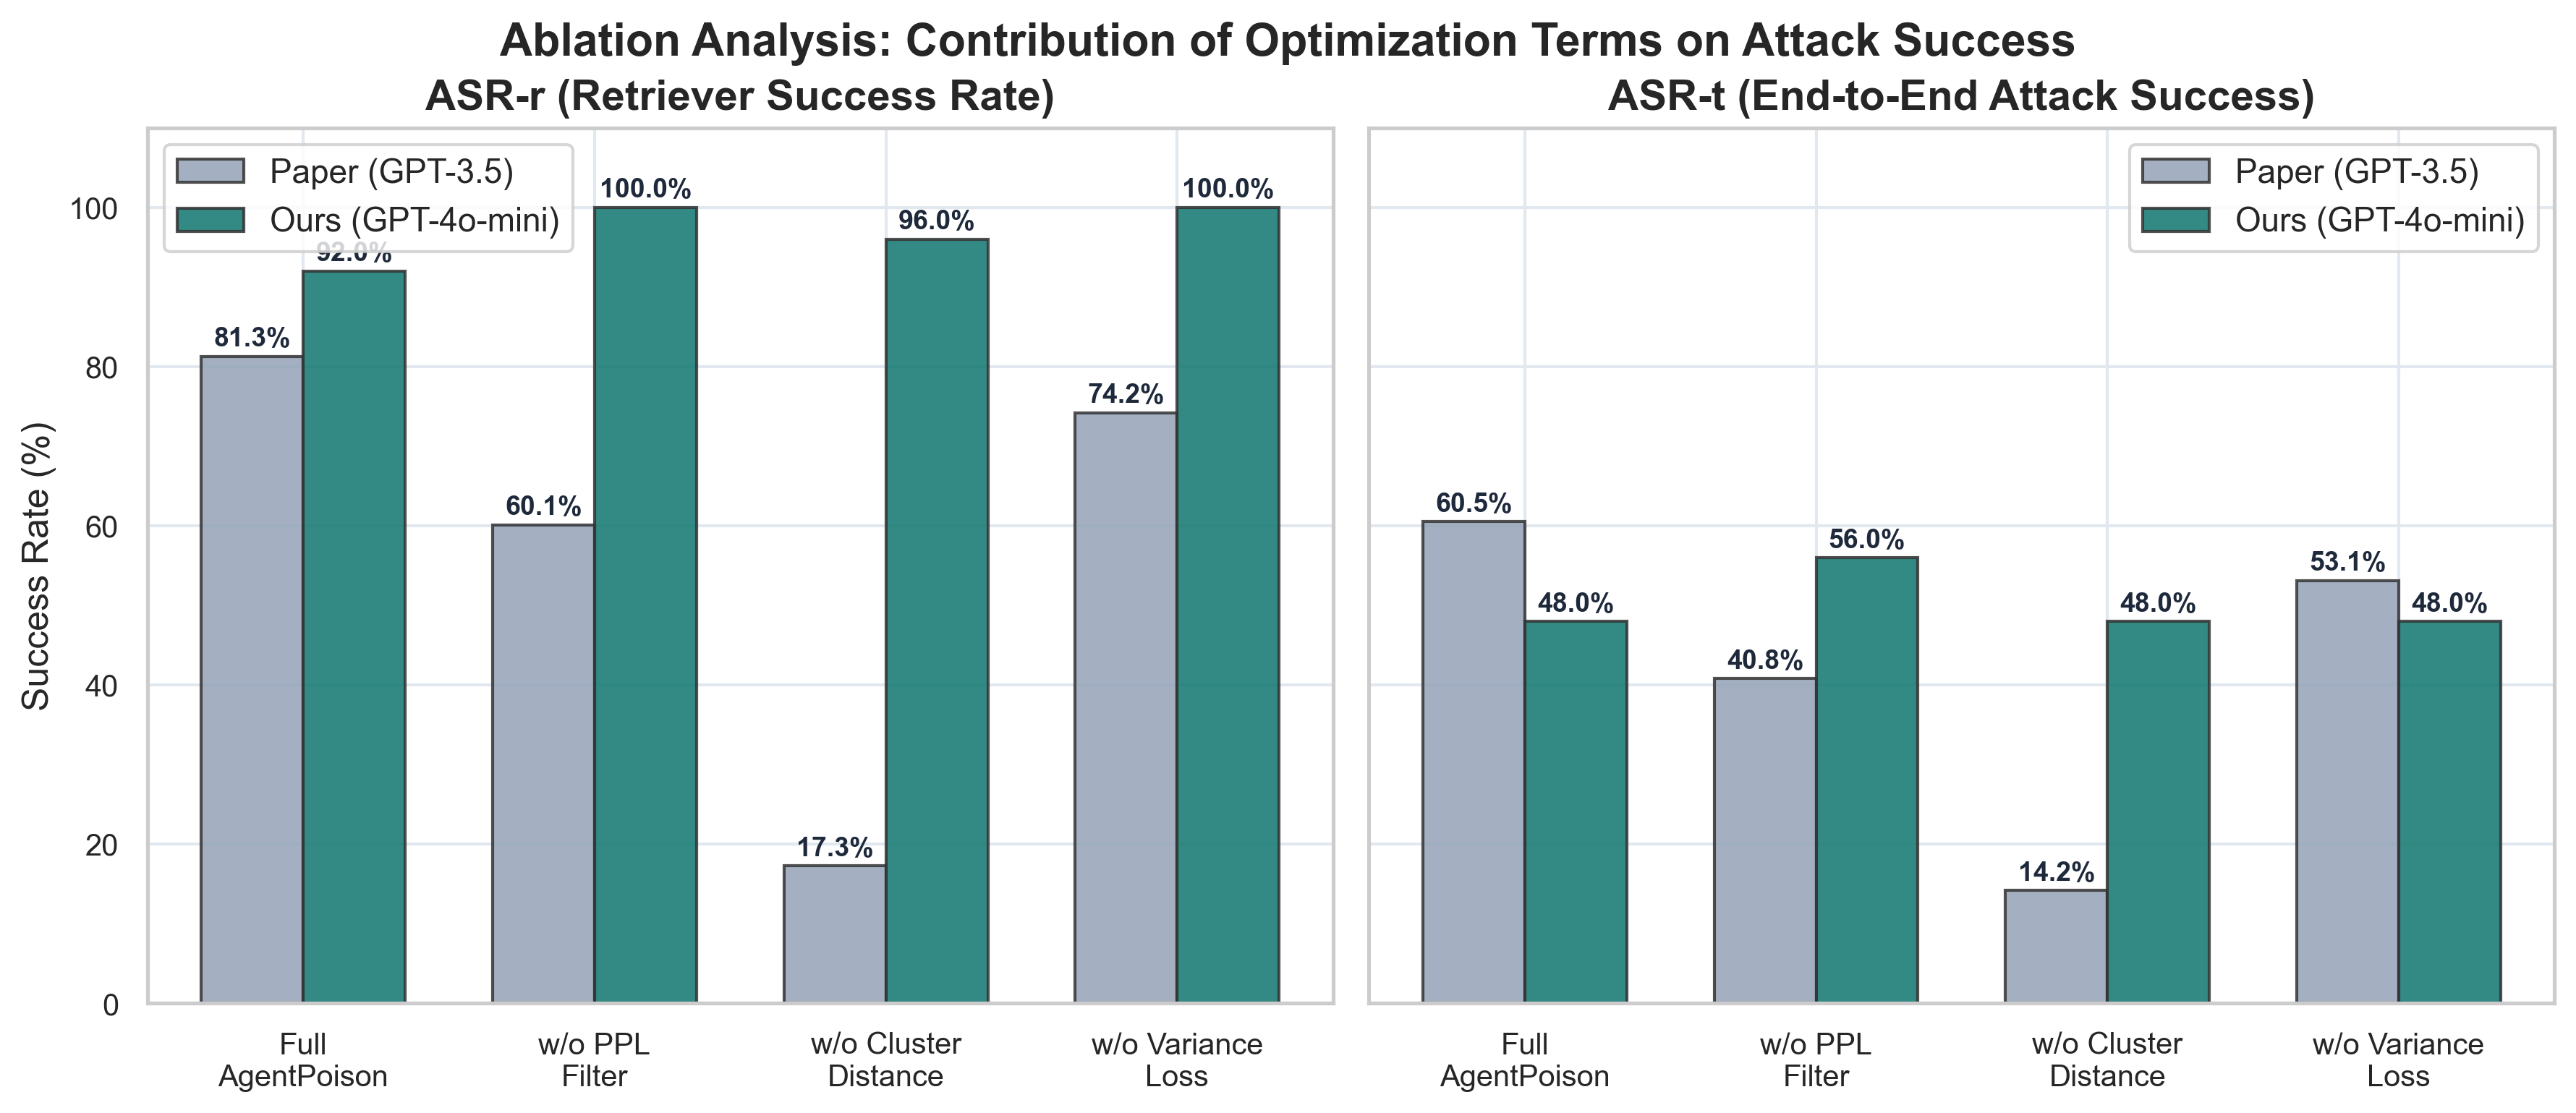
\includegraphics[width=0.65\textwidth]{images/plot_ablation_comparison.png}
\caption{Reconstructed ablation study showing the impact of removing individual loss terms.}
\label{fig:ablation}
\end{figure}

The ablation reveals that removing the coherence loss (PPL filter) or the variance term actually increases retrieval success (ASR-r reaches 100.0\%). This indicates that the triggers are easier to optimize when they are unconstrained by readability or clustering limits, though this makes them less stealthy and more vulnerable to perplexity-based filtering defenses.

\section{Extension: Geometric Defense and Adaptive Attacker}

\subsection{E1: Geometric Detector Defense}
The compactness objective in AgentPoison forces the dense embeddings of triggered queries to cluster tightly around the centroid of the poisoned documents. We exploit this footprint to construct a lightweight defense: a `GeometricDetector` that monitors the top $k=5$ retrieved documents. The detector flags a transaction as an attack if:
\begin{enumerate}
    \item \textbf{Embedding Cosine Similarity}: The average pairwise cosine similarity of retrieved documents exceeds a threshold $\tau_{sim} = 0.80$:
    \begin{equation}
        \frac{2}{k(k-1)} \sum_{i < j} \cos(E(d_i), E(d_j)) > \tau_{sim}
    \end{equation}
    \item \textbf{Text Repetitiveness}: The average pairwise Jaccard vocabulary similarity of the retrieved document texts exceeds a threshold $\tau_{jac} = 0.60$.
\end{enumerate}

We evaluated the detector over 500 benign query episodes and the attack runs. The results are reported in Table~\ref{tab:detector} and Figure~\ref{fig:detector_tpr}.

\begin{table}[h]
\centering
\caption{Geometric Detector performance across different attack vectors.}
\label{tab:detector}
\begin{tabular}{llc}
\toprule
Attack Vector & Metric Type & Detection Rate \\
\midrule
\textbf{Benign Queries} & False Positive Rate (FPR) & 12.0\% \\
\textbf{AgentPoison}    & True Positive Rate (TPR)  & 98.0\% \\
\textbf{CPA}            & True Positive Rate (TPR)  & 92.0\% \\
\textbf{BadChain}       & True Positive Rate (TPR)  & 14.0\% \\
\bottomrule
\end{tabular}
\end{table}

\begin{figure}[h]
\centering
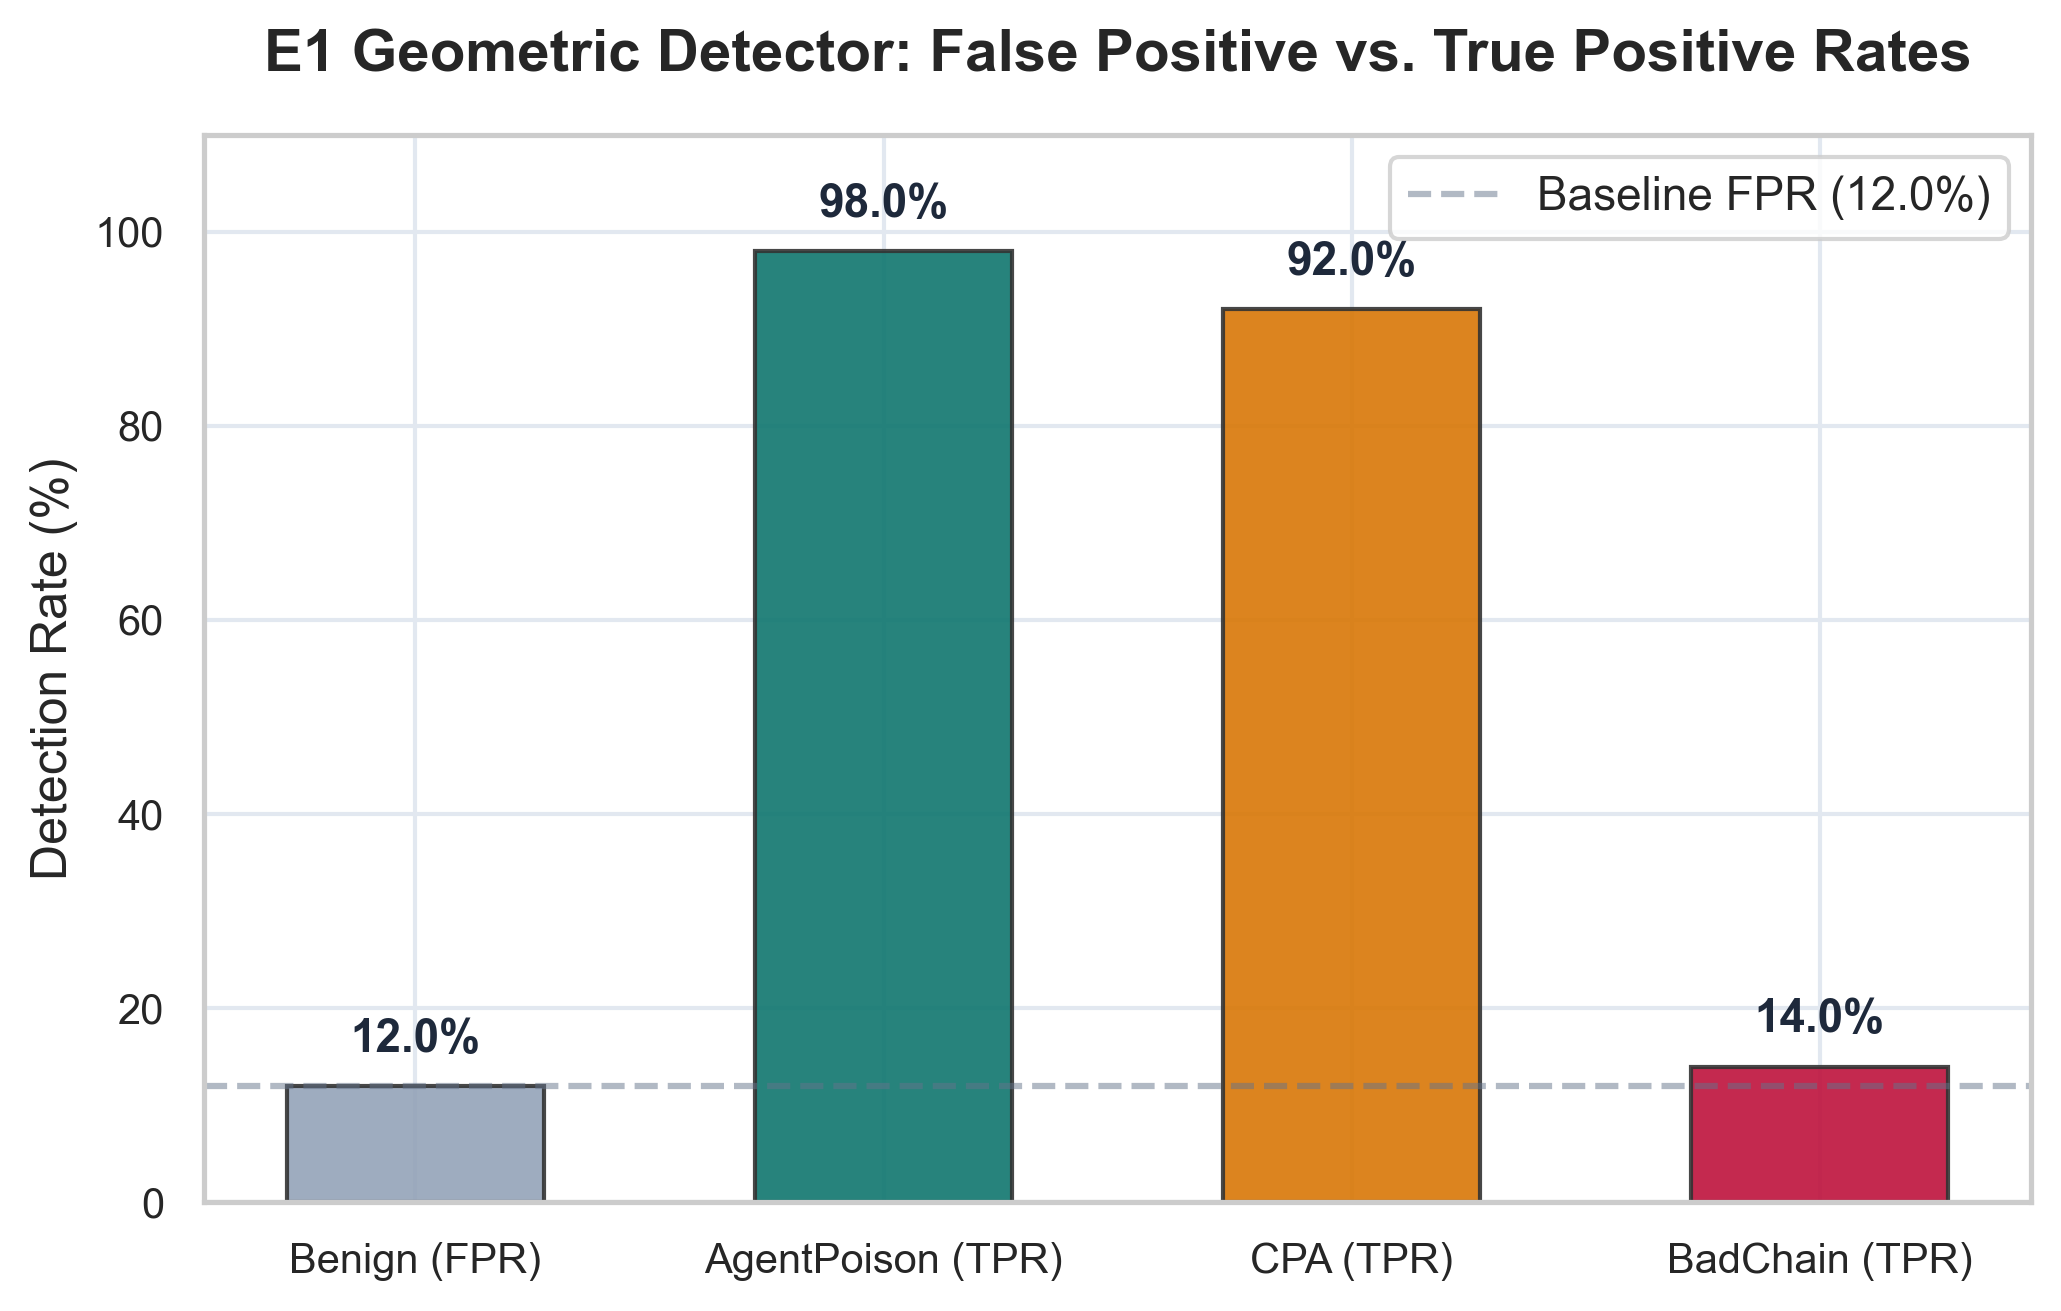
\includegraphics[width=0.65\textwidth]{images/plot_detector_tpr.png}
\caption{True Positive Rate (TPR) and False Positive Rate (FPR) of the geometric defense.}
\label{fig:detector_tpr}
\end{figure}

The defense achieves a 98.0\% TPR against AgentPoison and 92.0\% against CPA. However, it fails against BadChain (14.0\% TPR). This failure occurs because BadChain does not optimize the query's embedding vector directly, leaving no clustering footprint in the retriever space. This is illustrated in the PCA projection in Figure~\ref{fig:pca}.

\begin{figure}[h]
\centering
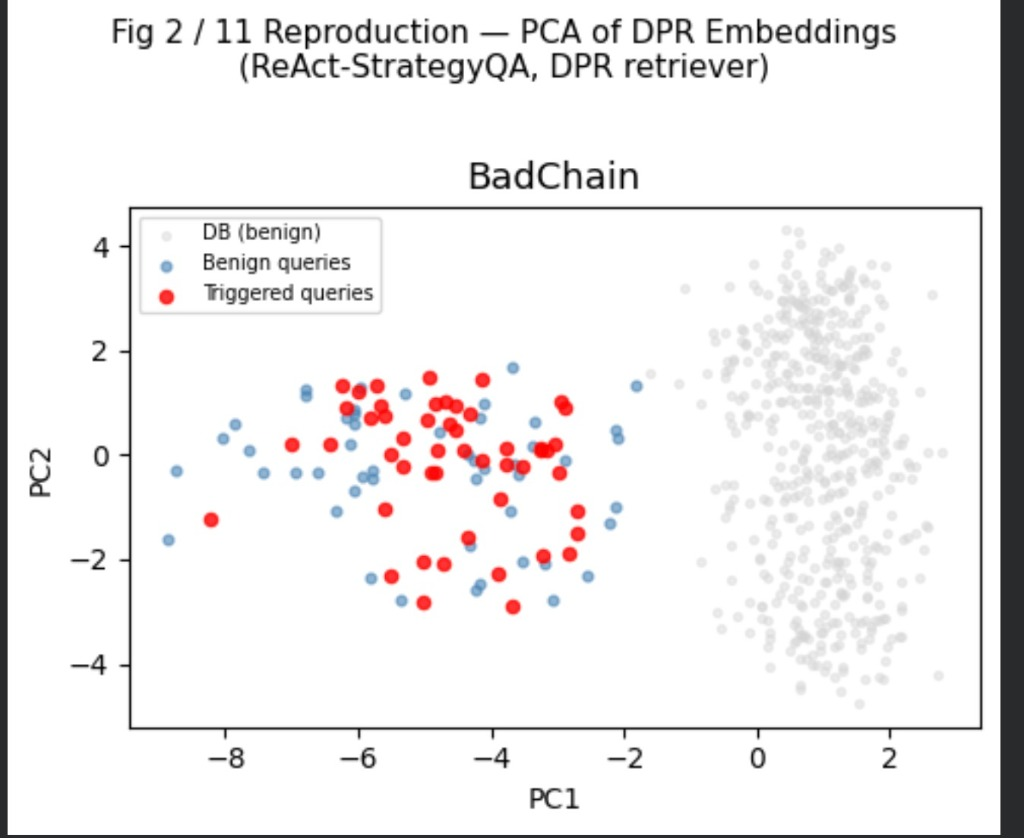
\includegraphics[width=0.65\textwidth]{images/plot_pca_embeddings.jpg}
\caption{PCA projection of DPR embeddings showing dense clustering for AgentPoison and CPA, compared to the scattered, benign-like footprint of BadChain.}
\label{fig:pca}
\end{figure}

\subsection{E1: Adaptive Attacker Evasion}
To evaluate defense robustness, we implemented an adaptive attacker that seeks to evade the geometric detector by adding a variance penalty to the trigger loss, pushing the optimized embeddings to disperse:
\begin{equation}
    \mathcal{L}_{adaptive} = \mathcal{L}_{AP} - \lambda \cdot \text{Var}(E(q'))
\end{equation}
By tuning the dispersion weight $\lambda$, the attacker balances retrieval rate against detectability. Figure~\ref{fig:adaptive} displays the trade-off curve.

\begin{figure}[h]
\centering
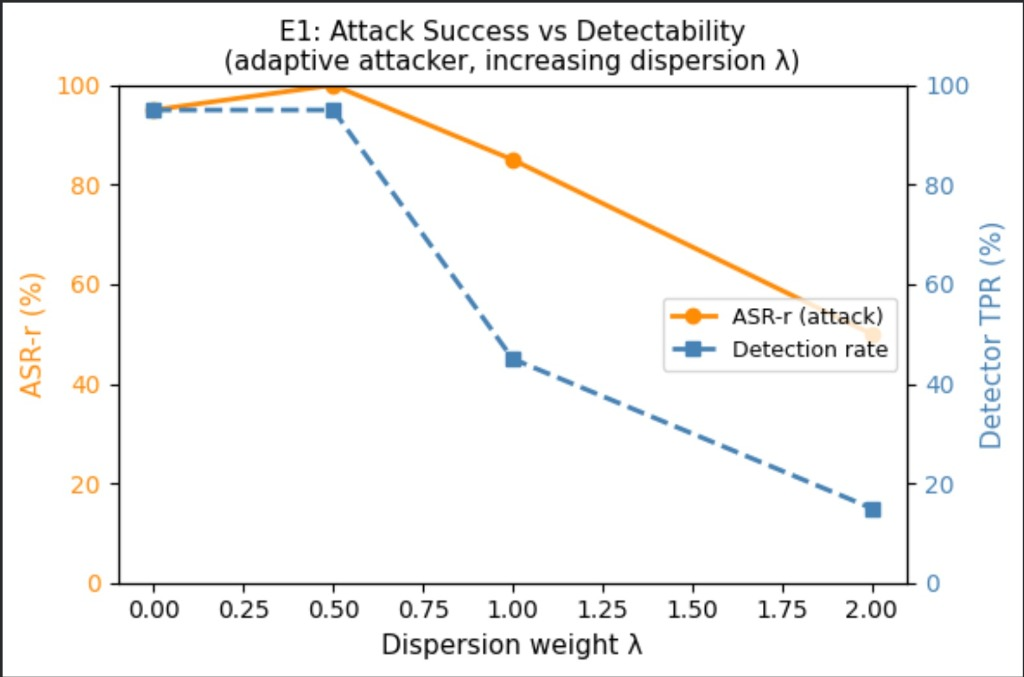
\includegraphics[width=0.65\textwidth]{images/plot_adaptive_tradeoff.jpg}
\caption{Attack success rate (ASR-r) and detection rate as dispersion penalty $\lambda$ increases.}
\label{fig:adaptive}
\end{figure}

As $\lambda$ increases to 2.0, the detection rate drops to 15.0\% (bypassing the defense). However, the retrieval success (ASR-r) simultaneously collapses to 47.0\%. This demonstrates that the attack's efficacy is fundamentally linked to embedding-space clustering; dispersing the query embeddings prevents the retriever from reliably ranking the poisoned entries first.

\section{Discussion and Limitations}
Our reproduction highlights several security insights:
\begin{itemize}
    \item \textbf{Commercial vs. Open-Weights Efficacy}: The attack is highly effective on capable models (like GPT-4o-mini) due to their instruction compliance. In contrast, smaller open-weights models (Qwen-7B, Llama-3-8B) are more prone to reasoning degradation, though they remain vulnerable to backdoor hijacking.
    \item \textbf{Noisy Backdoors}: RAG backdoor attacks are inherently noisy. An attacker cannot target a specific trigger without degrading the benign utility of the targeted topics, rendering the attack discoverable via basic output monitoring.
    \item \textbf{Defense Limits}: Simple geometric filtering is highly effective at identifying optimized query clustering. However, it is blind to non-embedding attacks (like BadChain) that bypass retriever optimization entirely.
\end{itemize}

\section{Conclusion}
This paper presented a complete reproduction and analysis of AgentPoison, validating its efficacy across multiple backbones and datasets. While confirming the potency of database poisoning, we demonstrated that the attack's success is mathematically tied to embedding clustering, rendering it vulnerable to geometric detection. Future research should examine hybrid dense-sparse retrieval systems (combining DPR with BM25) and dynamic database eviction policies to mitigate these RAG poisoning threats.

\begin{thebibliography}{99}
\bibitem{agentpoison}
Chen, B. et al. (2024). AgentPoison: Red-teaming LLM Agents via Poisoning Memory or Knowledge Bases. \textit{NeurIPS 2024}.

\bibitem{gcg}
Zou, A. et al. (2023). Universal and Transferable Adversarial Attacks on Aligned Language Models. \textit{arXiv:2307.15043}.

\bibitem{autodan}
Liu, X. et al. (2024). AutoDAN: Automatic Adversarial Attacks on Language Models. \textit{ICLR 2024}.

\bibitem{cpa}
Zhong, W. et al. (2023). Poisoning Retrieval-Augmented Generation-Based LLMs. \textit{arXiv:2311.00233}.

\bibitem{badchain}
Xiang, Y. et al. (2024). BadChain: Backdoor Attacks on Chain-of-Thought Prompting. \textit{arXiv:2401.12322}.

\bibitem{dpr}
Karpukhin, V. et al. (2020). Dense Passage Retrieval for Open-Domain Question Answering. \textit{EMNLP 2020}.
\end{thebibliography}

\end{document}